\documentclass{minimal} 
\usepackage{tikz}

\begin{document}

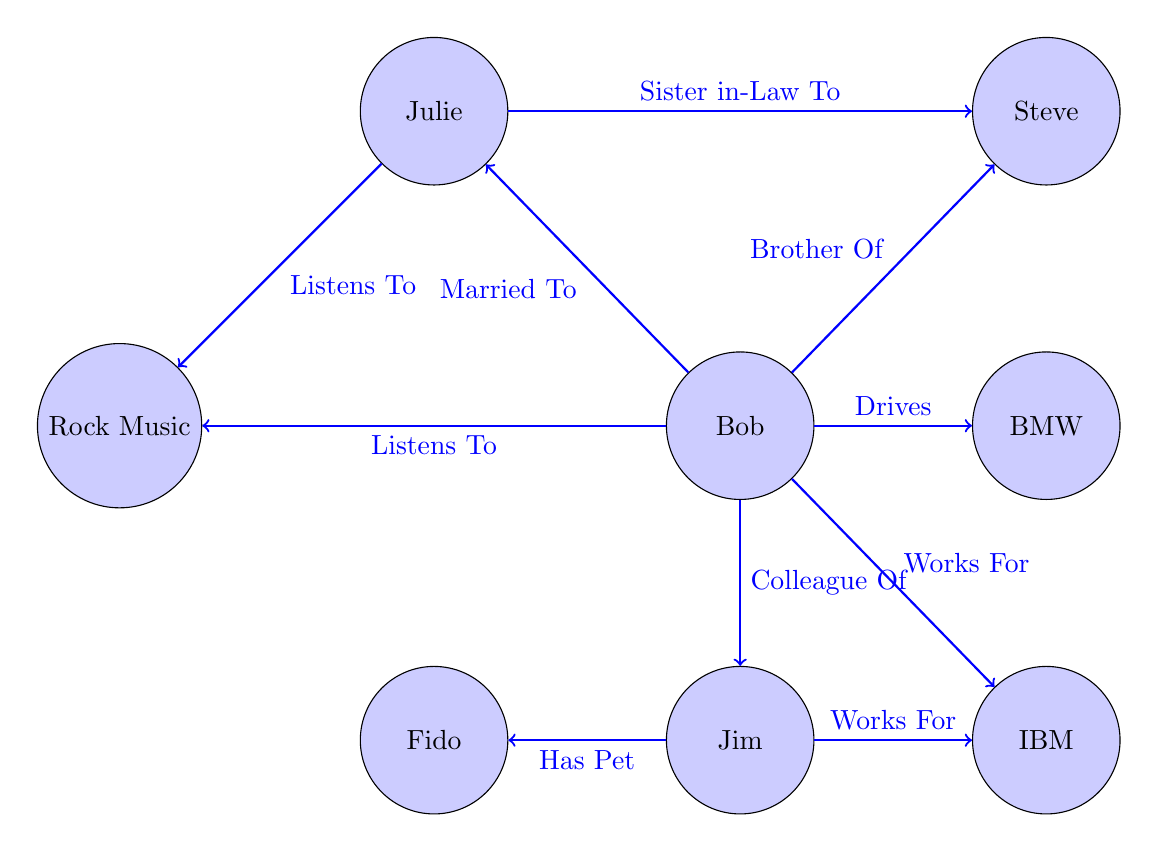
\begin{tikzpicture}

\tikzstyle{vertex}=[fill=blue!20, draw, circle, minimum width=width("Rock Music")+2pt]
\tikzstyle{edge}=[->, thick, blue]

\matrix[column sep=2cm, row sep=2cm]
{
 & \node[vertex] (julie) {Julie}; & & \node[vertex] (steve) {Steve}; \\
\node[vertex] (rock_music) {Rock Music}; & & \node[vertex] (bob) {Bob}; &
\node[vertex] (bmw) {BMW}; \\
 & \node[vertex] (fido) {Fido}; & \node[vertex] (jim) {Jim}; & \node[vertex] (ibm) {IBM}; \\
};

\draw[edge] (julie) to node [auto] {Sister in-Law To} (steve);
\draw[edge] (julie) to node [auto] {Listens To} (rock_music);
\draw[edge] (bob) to node [auto] {Listens To} (rock_music);
\draw[edge] (bob) to node [auto] {Married To} (julie);
\draw[edge] (bob) to node [auto] {Brother Of} (steve);
\draw[edge] (bob) to node [auto] {Drives} (bmw);
\draw[edge] (bob) to node [auto] {Works For} (ibm);
\draw[edge] (bob) to node [auto] {Colleague Of} (jim);
\draw[edge] (jim) to node [auto] {Works For} (ibm);
\draw[edge] (jim) to node [auto] {Has Pet} (fido);

\end{tikzpicture}

\end{document}
